\documentclass[11pt]{article}
\usepackage{../../cs70}
%\usepackage{../../markup}
\usepackage{color}
\newif\ifsolutions
\solutionsfalse
\def\title{Homework 3}
\begin{document}
\maketitle

\vspace{0.5em}
{\Large{\textbf{This homework is due Feb 10 2014, at 12:00 noon.}}}



\begin{qunlist}

\qns{A tiling problem} \\
You are given three kinds of tiles, \textbf{A,B,C} of dimensions $1 \times 2$, $2 \times 1$
and $2 \times 2$ respectively (as shown in the figure below).
\textit{Note that rotations of the tiles are not allowed, so tiles \textbf{A} and \textbf{B} are NOT the same!}

\begin{figure}[tile]
\centering
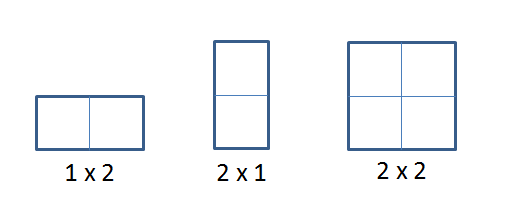
\includegraphics[scale=0.6]{resources/figures/tile.png}
\end{figure}

Your goal is to tile a board of dimension $2 \times n$, and you are interested in the number of
tiling configurations possible using the three types of tiles given. \\
Let $T_n$ denote the number of tiling configurations for a board of dimension $2 \times n$.
\begin{itemize}
\item[(a)] Show the base cases of this problem by direct enumeration.

\ifsolutions
\textcolor{blue}{
\textbf{Solutions:} $T_1 = 1$ as there is exactly one way to tile a $2 \times 1$ board, using tile \textbf{B}.
A $2 \times 2$ board can be tiled in exactly three different ways using the tiles \textbf{AA,BB} and \textbf{C},
so $T_2 = 3$.
}
\fi

\item[(b)] 


\item[(c)] Prove by induction that for all $n \geq 1$
\[ T_n = \frac{2^{n+1}+(-1)^n}{3} \]. 

\ifsolutions
\textcolor{blue}{
\textbf{Solutions:} 
}
\fi

\end{itemize}



%\qns{Title NA} \\
%Let $x,y$ be real numbers such that the numbers $x+y$, $x^2+y^2$, $x^3+y^3$, and $x^4+y^4$ are integers. \\ 
%Prove that for all positive integers $n$, the number $x^n + y^n$ is an integer.
%
%\ifsolutions
%\textbf{Solutions:}
%Use strong induction. Use the identity
%\[ x^{k+1} + y^{k+1} = (x+y)(x^k + y^k) - xy(x^{k-1} + y^{k-1}) \]
%
%We are given that $x+y$ is an integer, and by our inductive hypothesis $x^k + y^k$ and $x^{k-1} + y^{k-1}$ 
%are also both integers. So we need to show that $xy$ is an integer.  This can be shown because:
%\[ x^3 + y^3 = (x+y)(x^2+y^2) - xy(x+y) \]
%
%So our base cases are $n=5$ and $n=6$.  After that we can use strong induction.
%\fi



\qns{Title NA} \\
Define the following sequence: $a_1 =2$, $a_2 = 3$ and $a_k = a_{k-1} \cdot a_{k-2}$ for all $n \geq 3$. \\ 
Does the sum 
\[ A_n = \sum_{k=1}^n \frac{1}{a_k} \]

diverge (i.e. approach infinity) as $n \to \infty$, or does it converge to a finite number?  
Prove why or why not.
{\em Hint: plot $A_n$, and think about discussion 2b.}

\ifsolutions
\textbf{Solutions:}
It does converge. We can first use strong induction to prove the claim
\[ a_k > 2^k, \quad \forall k \geq 4 \] 

For the base cases we have $a_4 = a_3 \cdot a_2 = 6 \cdot 3 = 18 > 2^4$ 
and $a_5 = a_4 \cdot a_3 = 18 \cdot 6 = 108 > 2^5$. Then for the inductive step we have
\[ a_{k+1} = a_k \cdot a_{k-1} > 2^k \cdot 2^{k-1} = 2^{2k-1} > 2^{k+1} \]

Therefore:
\[ \sum_{k=4}^n \frac{1}{a_k} < \sum_{k=4}^n \frac{1}{2^k} \]

Since the RHS converges as $n \to \infty$, we know the LHS converges.  
Adding a constant (i.e. the first three terms) does not change the fact that it converges.
\fi



\qns{Title NA} \\ 
Given a natural number $n$, can the number $1$ be produced 
by repeatedly applying the function:
\[ f(n) = \left\{ \begin{array}{cl} n/4 & \text{if $n$ is divisible by 4} \\
(n+2)/4 & \text{if $n$ is even but not divisible by 4} \\
3n - 1 & \text{if $n$ is odd} \end{array} \right. \]
Prove why or why not.

\ifsolutions
\textbf{Solutions:}
You can always get to 1. We can prove this by strong induction. If $n=1$, we are done.  If $n=2$, we add 2 and divide by 4, and then are done.  For our inductive hypothesis, we assume we can get to 1 from any number less than $n$. Then if $n$ is dividible by 4, dividing $n$ by 4 reduces the problem to one we have already solved.  If $n$ is divisible by 2 but not 4, $(n+2)/4 < n$, so we've again reduced the problem to one we have already solved. \\

So the remaining case is if $n$ is odd.  In this case, $3n-1$ will be even, so then we would either divide by 4, or add 2 and divide by 4, in either case $(3n-1)/4$ and $(3n+1)/4$ are both less than $n$ if $n \geq 2$.
\fi



\qns{Let's grade proofs!} \\
For each of the induction ``proofs'' below, say whether you think the proof is correct or not.
If you think the proof is incorrect, explain \textit{clearly} and \textit{concisely} where the logical error lies.
If you think the proof is correct, you do not need to give any explanation. \\
\textit{Recall that simply saying the inductive hypothesis is false is not a valid explanation.}

\begin{itemize}
\item[(a)] \textbf{Claim:} $\forall n \in \N$ , $n^2 \leq n$. \\
\textbf{Proof:} \\
Base case: for $n = 1$, the claim is $1^2 \leq 1$, which is true. \\
Induction hypothesis: Assume that $k^2 \leq k$. \\
Inductive step: We need to show that \[ (k+1)^2 \leq k+1\] \\
Working backwards we see that \[ k^2 \leq (k+1)^2 - 1 \leq (k+1) - 1 = k \] \\
So we get back to our original hypothesis which is assumed to be true.\\
Hence, for every $n \in \N$, we know that $n^2 \leq n$. 

\ifsolutions
\textbf{Solutions:}
\fi


\item[(b)]\textbf{Claim:} $\forall n \in \N$ , $7^n = 1$. \\
\textbf{Proof:} \\
Base case: Certainly $7^0 = 1$. \\
Induction hypothesis: Assume that $7^j = 1$ for all $0\leq j \leq k$.\\
Inductive step: We need to prove that $7^{k+1} = 1$, and we have,
\[ 7^{k+1} = \frac{7^k \cdot 7^k}{7^{k-1}} = \frac{1 \cdot 1}{1} = 1\]

Hence, by the Principle of Strong Induction, $7^n = 1$ for all $n \in \N$.

\ifsolutions
\textbf{Solutions:}
\fi


\item[(c)]\textbf{Claim:} $\forall n \in \N$, if $n \geq 4$, then $2^n < n!$. \\
\textbf{Proof:} \\
Base case: $2^4 = 16$ and $4! = 24$, so the claim is true for $n=4$. \\
Induction hypothesis: Assume $n \geq 4$ and $2^n < n!$. \\
Inductive step: \[ 2^{n+1} = 2(2^n) < 2(n!) < (n+1)(n!) = (n+1)!\]
So we have shown that $2^{n+1} < (n+1)!$ and this completes the proof.

\ifsolutions
\textbf{Solutions:} This proof is correct.
\fi


\item[(d)]\textbf{Claim:} $\forall x,y,n \in \N$, if $\max(x,y) = n$, then $x \leq y$. \\
\textbf{Proof:} \\
Base case: For $n=0$, if $\max(x,y) = 0$ and $x,y \in \N$, then $x=0, y=0$, hence $x \leq y$. \\
Induction hypothesis: Assume that whenever we have $\max(x,y) = n$, $x \leq y$ mush hold. \\
Inductive step: We must prove that if $\max(x,y) = n+1$, then $x \leq y$. \\
Suppose $x,y$ are such that $\max(x,y) = n+1$, then it follows that $\max(x-1,y-1) = n$. \\
So by the inductive hypothsis, $x-1 \leq y-1  \implies x \leq y$, completing the proof.

\ifsolutions
\textbf{Solutions:}
\fi


\end{itemize}




\qns{Marty's Marriage Mistake} \\ 

\begin{itemize}
\item[(a)] My friend Marty and I run a match-making business. We receive preference lists from men and women and use the same propose-and-reject algorithm you covered in class. Marty, being a traditionalist, insists on having the men propose, while I, in a subtle attempt to subvert the patriarchy, have the women propose. Prove that if both Marty and I come up with the same pairings, there is no other possible stable pairing (i.e. a pairing with no rogue pairs)

\item[(b)] While I'm on vacation, things get a little disorganized. Marty loses track of some of the preference lists. He is too embarrassed to ask the women for their preferences again. He knows the following preferences:

\begin{center}
\begin{tabular}{|c|ccc|}\hline 
Man&\multicolumn{3}{|c|}{Women}\\\hline 
A&1&2&3\\\hline 
B&3&2&1\\\hline 
C&1&3&2\\\hline
\end{tabular} 
\hspace{2cm}
\begin{tabular}{|c|ccc|}\hline 
Woman&\multicolumn{3}{|c|}{Men}\\\hline 
1&?&?&?\\\hline 
2&A&B&C\\\hline 
3&?&?&?\\\hline
\end{tabular}
\end{center}
   
   Marty decides to assume that 1 and 3 would have the same preferences as 2. Show the steps of Marty running the propose-and-reject algorithm (with men proposing). Please indicate the final pairing clearly and note how many days it took to reach that pairing.

\item[(c)] When I come back from my vacation, Marty explains the previous situation. He smugly informs me that none of the couples have switched after he proposed a matching, and therefore there are no rogue pairs. Because of this, I shouldn't bother running the algorithm having women propose. I am not so certain that he is correct. After all, he ran the algorithm on incomplete data. I want to convince him that another pairing could exist. Show that (without changing any of the known preferences) there exists a list of preferences for 1 and 3 in which I would pair everyone with somebody different. Remember, in my version, I have the women propose.

\item[(d)] At the homework party, two of your friends attempt part c, above. 

Here is your first friend's work: 

\begin{center}
\begin{tabular}{|c|ccc|}\hline 
Woman&\multicolumn{3}{|c|}{Men}\\\hline 
1&A&?&?\\\hline 
2&A&B&C\\\hline 
3&?&?&?\\\hline
\end{tabular} 
\end{center}

Here is your second friend's work:

\begin{center}
\begin{tabular}{|c|ccc|}\hline 
Woman&\multicolumn{3}{|c|}{Men}\\\hline 
1&?&?&?\\\hline 
2&A&B&C\\\hline 
3&?&C&?\\\hline
\end{tabular}
\end{center}
 
 No matter how the rest of the preferences are filled out, these will result in invalid solutions to part c. Explain why.
\end{itemize} 
    



        
\qns{All is fair in love and adversaries} \\
\begin{itemize}
\item[(a)] It turns out that Marty has gotten his fair share of enemies over the years. We receive a stable marriage pairing, but one of his rivals has maliciously eliminated some of the preferences:

\begin{center}
\begin{tabular}{|c|ccc|}\hline 
Man&\multicolumn{3}{|c|}{Women}\\\hline 
A&X&1&X\\\hline 
B&X&X&X\\\hline 
C&3&X&X\\\hline
\end{tabular} 
\hspace{2cm}
\begin{tabular}{|c|ccc|}\hline 
Woman&\multicolumn{3}{|c|}{Men}\\\hline 
1&B&A&C\\\hline 
2&X&X&C\\\hline 
3&X&X&C\\\hline
\end{tabular}
\end{center}
        
        Luckily, we correctly guess a stable pairing is \{(A,1), (B,2), (C,3)\}. List all the possibilities of filling in the missing preferences such that the pairing we guessed is stable. 
        
\item[(b)] I begin to suspect that one of Marty's adversaries may have done worse than eliminate preferences. Some of the preferences may be switched! Marty isn't too worried. He says that if the adversary switches the order of only two of the preferences for one person, than it's possible our pairing (based on corrupted preferences) will still have no rogue couples. Assuming the information we received in part a is not corrupted, tell us which two preferences can be switched such that after Marty runs the propose-and-reject algorithm, he will get a pairing that is stable. (You should note it by index. For example, "The adversary switches A's 1st and 3rd preference").
        
\item[(c)] I tell Marty it's possible that even with just two preferences being switched, we could get a lot of rogue pairs. For an arbitrary stable marriage instance, how many rogue pairs could be generated by an adversary switching the order of two preferences for one person?
        
\item[(d)] Marty counters by suggesting some preferences are very stable. If an adversary looks at one person's preference list and switches it around to do the most damage possible, what are the least number of rogue pairs that will be generated? For a Stable Marriage problem with n men and women, describe this stable list of preferences.


\end{itemize}


\qns{College Admissions}\\
In the College Admissions Problem, we are given $n$ students and $m$ universites. Each university $u$ has some number, $q_u$ of slots, and we assume that the total number of students is larger than the total number of slots
(i.e. $\sum_{u=1}^m{q_u} < n$). Each student ranks the $m$ universities in order of preference, and each university ranks the $n$ students. Our goal is to find an assignment of students to slots(one student per slot) that is
\textit{stable} in the following sense:
\begin{itemize}
\item There is no student-university pair $(s,u)$ such that s prefers u to her allocated university and u prefers s to one of the students assigned to u.
\item There is no university u that prefers some unassigned student s to one of the students assigned to u.
\end{itemize}

Note that this problem is almost the same as the Stable Marriage Problem, with two differences: \\
(i)there are more students than slots; \\
(ii)each university generally has more than one slot.

\begin{itemize}
\item[(a)] Explain how to modify the Propose and Reject algorithm so that it finds a stable assignment of students to slots.

\item[(b)] Carefully state a version of the Improvement Lemma that applies to your algorithmm.

\item[(c)] Use your Improvement Lemma to give a proof taht your algorithm does indeed find a stable assignment.

\end{itemize}











\qns{Write your own problem} \\

Write your own problem related to this week's material and solve it. You may still work in groups to brainstorm problems, but each student should submit a unique problem. What is the problem? How to formulate it? How to
solve it? What is the solution?


\end{qunlist}

\end{document}



